\newpage
\section{Określenie wymagań szczegółowych}		%2
%Dokładne określenie wymagań aplikacji (cel, zakres, dane wejściowe) – np. opisać przyciski, czujniki, wygląd layoutu, wyświetlenie okienek. Opisać zachowanie aplikacji – co po kliknięciu, zdarzenia automatyczne. Opisać możliwość dalszego rozwoju oprogramowania. Opisać zachowania aplikacji w niepożądanych sytuacjach.

\hspace{0.60cm}Firma serwisowa Ttest pragnie aby stworzyć aplikację mobilną do testowania czujników, która byłaby zachowana w sposób minimalistyczny i intuicyjny. Przejrzysta i prosta budowa menu, miałaby na celu usprawnić szukanie odpowiednich komponentów. Firma posiada również logo, które powinno zawierać się w projekcie, jak i niebieskie akcenty (np. przyciski) który powinny towrzyszyć aplikacji ponieważ jest to kolor kojarzony z firmą. \newline

Jednym z kluczowych zadań jest stworzenie aplikacji w sposób jak najbardziej przejrzysty, do tego celu użyjemy ikonek, które w prosty i szybki sposób nakierują nas na odpowiedni komponent. Przykładem może być latarka; chcąc przetestować jej działanie wystarczy wybrać ikonkę która będzie przedstawiała latarkę. Po jej naciśnięciu zostaniemy przekierowani do strony z testem. Oprócz testowania czujników, zapewnimy moduł odpowiedzialny za posdumowanie wszystkich przeprowadzonych testów. Zapewniamy również zawarcie logotypu i zachowania layoutu aplikacji w niebieskich kolorach, sprawimy by layout w całości był jak najbardziej intuicyjny i zachowany w minimalistyczny sposób (brak jaskrawych kolorów, duże przejrzyste przyciski, okienka pop-up z wiadomościami o przebiegu testu). Postaramy się aby komponenty testujące takie jak: latarka, test dźwięku, tryb nocny i tym podobne; będą poprawnie spełniać swoje zadanie. Aplikacja zostanie napisana w programie Android Studio, natomiast język którym będziemy się posługiwać to: Java.\newline

Na obrazku \ref{rys:ikona} znajduje się logo, które będzie użyte jako ikonka aplikacji. Została ona stworzona przez zespoł naszych grafików, wraz z zakończeniem prac nad aplikacją, firma Ttest dodstanie pełne prawa do posługiwania się tym logotypem.
\begin{figure}[!hbt]
	\begin{center}
		
\includegraphics[angle=360, width=0.30\textwidth]{rys/punkt2/app_icon.png}
		\caption{Ikona aplikacji}
		\label{rys:ikona}
	\end{center}
\end{figure}

\newpage

Poglądowy zarys wyglądu menu znajduje się na obrazku \ref{rys:menu}. Jest to jedynie zarys layoutu, dlatego nie wszystkie z ukazanych na nim testów będą znajdować się w finalnej aplikacji. \newline

\begin{figure}[!hbt]
	\begin{center}
		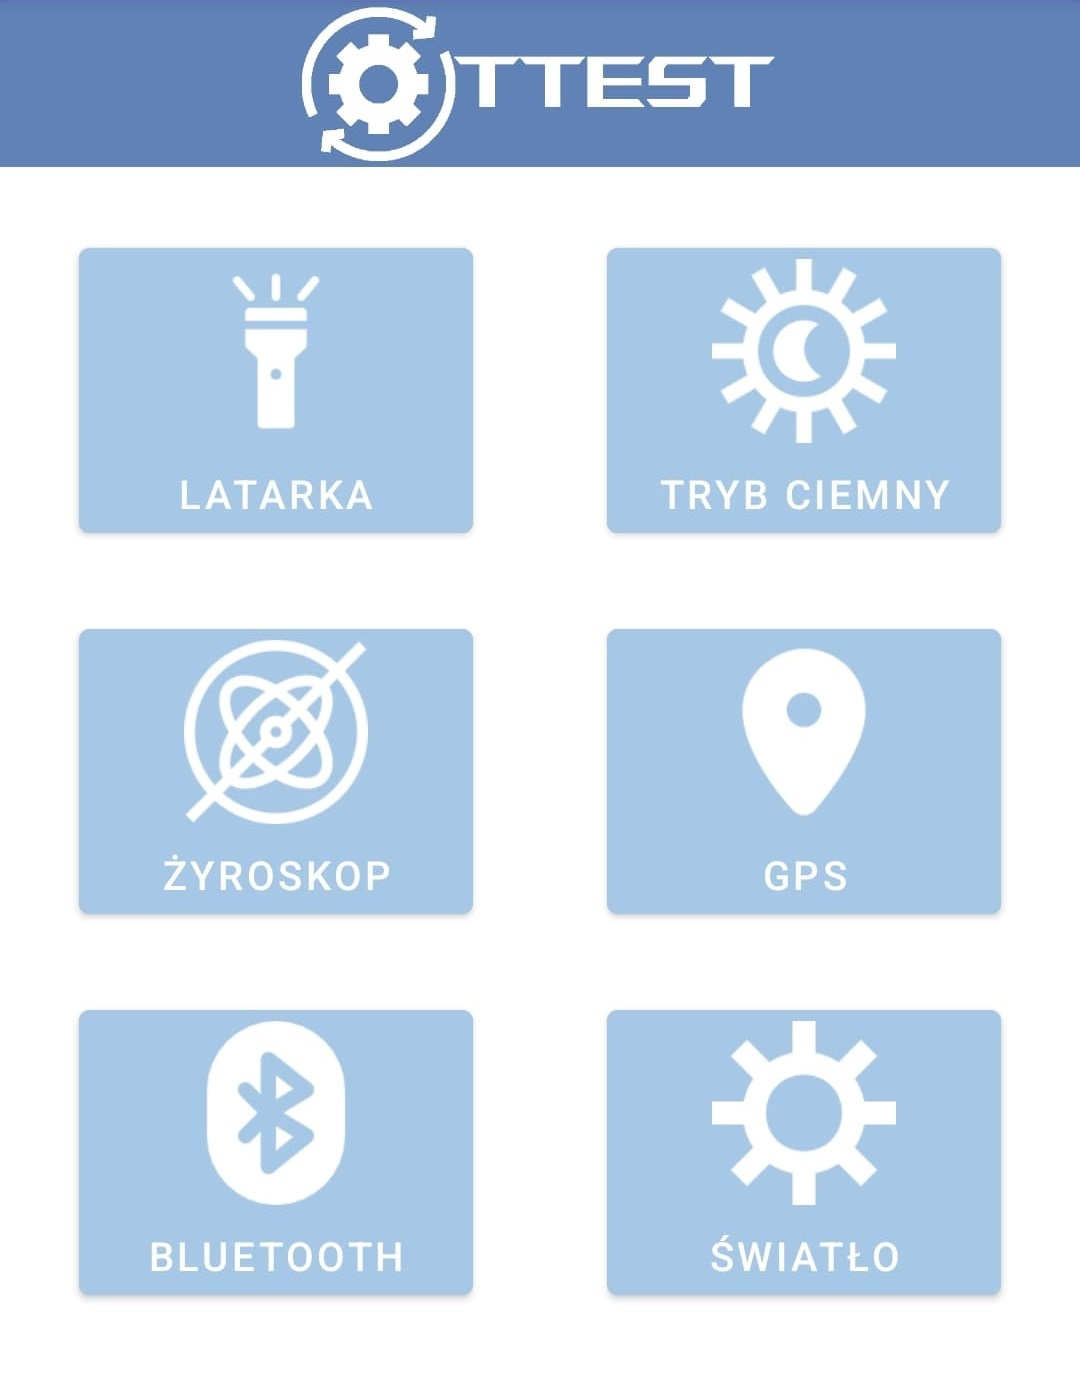
\includegraphics[angle=360, width=0.50\textwidth]{rys/punkt2/menu.jpg}
		\caption{Wygląd menu głównego}
		\label{rys:menu}
	\end{center}
\end{figure}

Tak jak już wspomnieliśmy powyżej postaramy się by każdy z czujników działał w należyty sposób; to znaczy by latarka poprzez kliknięcie przycisku włączała się i wyłączała. Test dźwięku pozwoli nam poprzez kliknięcie przycisku usłyszeć z głośników wydobywającą się melodię. Tryb nocny, który jest bardzo przydatną funkcją w telefonie szczególnie wieczorami gdy korzystamy z urządzeń mobilnych, zmieni kolorystykę z jasnej na ciemną. Przez tą funkcję jaka jest tryb ciemny nasze oczy nie są narażane na tak mocne światło, co sprawia, że czujemy większy komfort w użytkowaniu telefonów komórkowych. Kolejny czujnik jakim będzie GPS pozwoli nam w szybki sposób określić położenie w którym się znajdujemy. Test Wifi umożliwi spawdzenie połączenia z siecią, natomiast test mikrofonu sprawdzi się w sytuacji gdy na przykład pojawi się problem podczas rozmów telefonicznych. Test aparatu pozwoli wykonać zdjęcie oraz przetestować jakość wykonanego zdjęcia. \newline

\newpage

Do podsumowania wyników będzie prowadził nas jednej z przycisków znajdujących się w menu głównym. Podglądowy wyląd strony z wynikami znajduje się na obrazku \ref{rys:wyniki}. W miejscu "Marka i model telefonu" wyświetlą się informacje o telefonie na którym obecnie zostały przeprowadzanie testy. Do podsumowania testów zostaną użyte przyciski typu radio, które pozwalają na wybór tylko jednego przycisku z grupy: "Tak" albo "Nie. Kiedy zostanie naciśnięty przycisk "PODSUMUJ", ponieżej zostanie wyświetlona lista podsumowująca wszyskie przeprowadzone testy.

\begin{figure}[!hbt]
	\begin{center}
		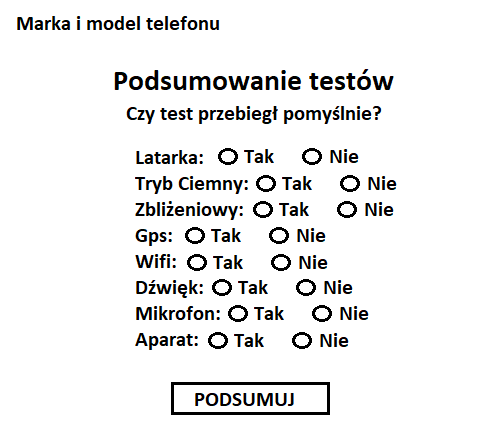
\includegraphics[angle=360, width=0.60\textwidth]{rys/punkt2/wyniki.png}
		\caption{Podsumowanie testów}
		\label{rys:wyniki}
	\end{center}
\end{figure}






